\mbox{$\displaystyle $\,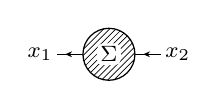
\begin{tikzpicture}[x=0.550cm, y=0.550cm, line width=0.450pt, baseline={([yshift=-0.6ex]0,0)}]
  \draw (0.000,0.000) -- (-0.600,0.000);
  \draw (0.000,0.000) -- (0.600,0.000);
  \draw (-0.600,0.000) -- (-1.200,0.000);
  \fill (-1.009,0.000) -- (-0.851,-0.068) -- (-0.902,0.000) -- (-0.851,0.068) -- cycle;
  \draw (0.600,0.000) -- (1.200,0.000);
  \fill (0.791,0.000) -- (0.949,-0.068) -- (0.898,0.000) -- (0.949,0.068) -- cycle;
  \fill[white] (0.000,0.000) circle (0.600);
  \draw[line width=0.248pt] (-0.588,0.119) -- (-0.119,0.588) (-0.599,-0.033) -- (0.033,0.599) (-0.580,-0.155) -- (0.155,0.580) (-0.541,-0.259) -- (0.259,0.541) (-0.489,-0.348) -- (0.348,0.489) (-0.424,-0.424) -- (0.424,0.424) (-0.348,-0.489) -- (0.489,0.348) (-0.259,-0.541) -- (0.541,0.259) (-0.155,-0.580) -- (0.580,0.155) (-0.033,-0.599) -- (0.599,0.033) (0.119,-0.588) -- (0.588,-0.119);
  \begin{scope}
  \clip (0.000,0.000) circle (0.600);
  \node[font=\footnotesize, inner sep=1.2pt, fill=white, rounded corners=2pt] at (0.000,0.000) {$\Sigma$};
  \end{scope}
  \draw (0.000,0.000) circle (0.600);
  \node[font=\footnotesize, inner sep=0pt, anchor=0] at (-1.290,0.000) {$x_{1}$};
  \node[font=\footnotesize, inner sep=0pt, anchor=180] at (1.290,0.000) {$x_{2}$};
\end{tikzpicture}}
